\section{\label{Simulation}Simulation Description}
In this section we provide details of the model. Subsection \ref{SpacePotentialAndField} describe how the space potential and electric field are calculated including the plasma sheath and in the RFEA region. Subsection \ref{IonTrajectory} describe the method to integrate the ion trajectories under the effect of the fields decribed in subsection \ref{SpacePotentialAndField}. Subsection \ref{IonCollision} describes the method to simulate ion collisions with the background gas. 

\subsection{\label{SpacePotentialAndField}Space Potential and Electric Field}
The space potential and electric field are calculated in two regions: the RFEA region, and the plasma sheath. The model is one-dimensional, therefore only space potential and electric field in the z-axis is calculated in these regions. In this geometry, the RFEA is located at $z \leq 0$ and its extension in the negative direction of the z-axis depends on the spaces between the grids and the collector; subsection \ref{RFEA}. The plasma sheath starts at $z=0$ and extends to the plasma, which is located at some $z_\text{plasma} > 0$. The location of the plasma sheath boundary edge depends on the plasma sheath model and is further described in subsection \ref{SheathModel}.   

\subsubsection{\label{RFEA}Retarding Field Energy Analyzer}
The RFEA modeled includes the standard four grids and collector plate~\cite{Hutchinson1987}. These are identified as G$_0$, G$_1$, G$_2$, G$_3$, C. The first grid, G$_0$, faces the plasma and is at the same potential as the electrode that bounds the plasma discharge. In this model, the voltage of G$_0$ is set to zero. The second grid, G$_1$ is typically biased negative respect to G$_0$ to repel electrons from the plasma discharge. The model does not include electrons, however, this grid is included to simulate the electric field that affects the motion of ions between G$_0$ and G$_1$. The third grid, G$_2$, is used to discriminate ions by setting the voltage of G$_2$ positive relative to G$_0$. The voltage of G$_2$ is typically swept from zero to a large voltage to limit the ion current to the collector and generate the RFEA characteristic voltage-current curve. The fourth grid, G$_3$, is used to repel secondary electrons that may be emitted by the collector due to ion impact. This grid is usually biased slightly negative relative to the voltage applied to the collector. Again, the model does not include electrons, however, it is included to simulate the electric field between G$_3$ and the collector that afect the ion trajectories. Finally, the last electrode in the RFEA is the collector, C, which is biased somewhat negative relative to the first grid, G$_0$.

The model assumes that the grids and non-dimensional; i.e. zero thickenss. This differs from actual RFEA devices where the grids are usually 40~$\mu$m thick (reference some publication by Impedans). Consequently, the model also neglects any lensing effects of non-zero thick grids~\cite{vandeVen2018,Buiter2018}. The distance between grids and the collector are defined in the model as multiples of 100~$\mu$m. In actual RFEA devices the grids are physically separated by sheets of Mica, 100$\mu$m thick each sheet. The arrangement of grids and spacers is known as the RFEA button stack. For instance, the standard RFEA button stack of a commercial device comprises two spacers between G$_0$ and G$_1$, three spacers between G$_1$ and G$_2$, three spacers between G$_2$ and G$_3$, and two spacers between G$_3$ and the collector C (reference impedans website Semion). This arrangement is therefore known as a 2332 button stack. The model can simulate the RFEA with any combination of button stack arragements expressed as multiples of the basic spacer. 

Besides lensing effects, not included in this model, actual grids are not entirely transparent and a fraction of ions moving through the RFEA are collected by the grids. The transparency of the grids depends on the ion energy and may vary due to the lensing effect. While the model presented here does not simulate these effects it includes a simple transparency factor setting. The user can set this number to any value from 0 to 100\%. The transparency setting is common to all grids; i.e., the transparency of grids cannot be set individually.     

The space potential between grids is calculated by linear interpolation. Similarly, the electric field between grids is calculated as the potential difference between each grid pair divided by the distance. Figure~\ref{fig:DCpotentialField} shows the space potential and electric field in the RFEA for grid voltage settings G$_0$=0, G$_1$=-60, G$_2$=250, G$_3$=-70, and C=-60~V. The location of the grids and collector is indicated with vertical dashed lines. 


\subsubsection{\label{SheathModel}Sheath Model}
The space potential and electric field in the sheath region of the plasma is determined from the Child Law sheath model for direct-current sheath~\cite{Lieberman2005}, and from the analytical solution of capacitive radio-frequency sheath for alternate-current sheath~\cite{Lieberman1988}. 

The Child Law sheath size is calculated 
\begin{equation}
s_\text{Child Law} = \frac{\sqrt{2}}{3} \lambda_D \left( \frac{2 V_0}{T_e} \right)^{3/4}
\end{equation}
Where $\lambda_D$ is the Debye length
\begin{equation}
\lambda_D = \sqrt{ \frac{\epsilon_0 T_e}{e n_s} }
\end{equation}
Where $T_e$ is the electron temperature (in eV), $\epsilon_0$ is vacuum permittivity (in Farads/metre), $e$ is the basic electric charge (in Coulomb), and $n_s$ is the plasma density at the sheath edge (in m$^{-3}$).

The voltage in the Child Law sheath is given by
\begin{equation}
V_\text{Child Law}(z) = V_0 \left( 1 -  \left( 1 -\frac{z}{s_\text{Child Law}} \right)^{4/3} \right)
\end{equation}
Where the position variable, $z$, is given in metres, and where $V_0$ is the voltage of the plasma sheath edge relative to the bounding electrode at $z=0$. The voltage is null at $z=0$ and $V_0$ at $z=s_\text{Child Law}$. The plasma potential is positive relative to the electrode, therefore $V_0$ is positive.

The electric field (in V/m) is given by
\begin{equation}
E_\text{Child Law}(z) = -\frac{4}{3} \frac{V_0}{s_\text{Child Law}} \left( 1 - \frac{z}{s_\text{Child Law}}  \right)^{1/3}
\end{equation}
Note the field is null at $z=s_\text{Child Law}$ and negative otherwise in the sheath region. 

Figure~\ref{fig:DCpotentialField} shows the space potential and electric field for the DC sheath solution with a voltage across the sheath of 1000~V and plasma density $n_s = 10^{16}$~m$^{-3}$. Note that even for a small voltage at the discriminator grid G$_2$ (relative to the plasma potential) the electric fields within the RFEA are much higher than the electic field across the sheath due to the proximity between grids; i.e., ions experience substantially higher forces within the RFEA. 

\begin{figure}[htbp]
\centering
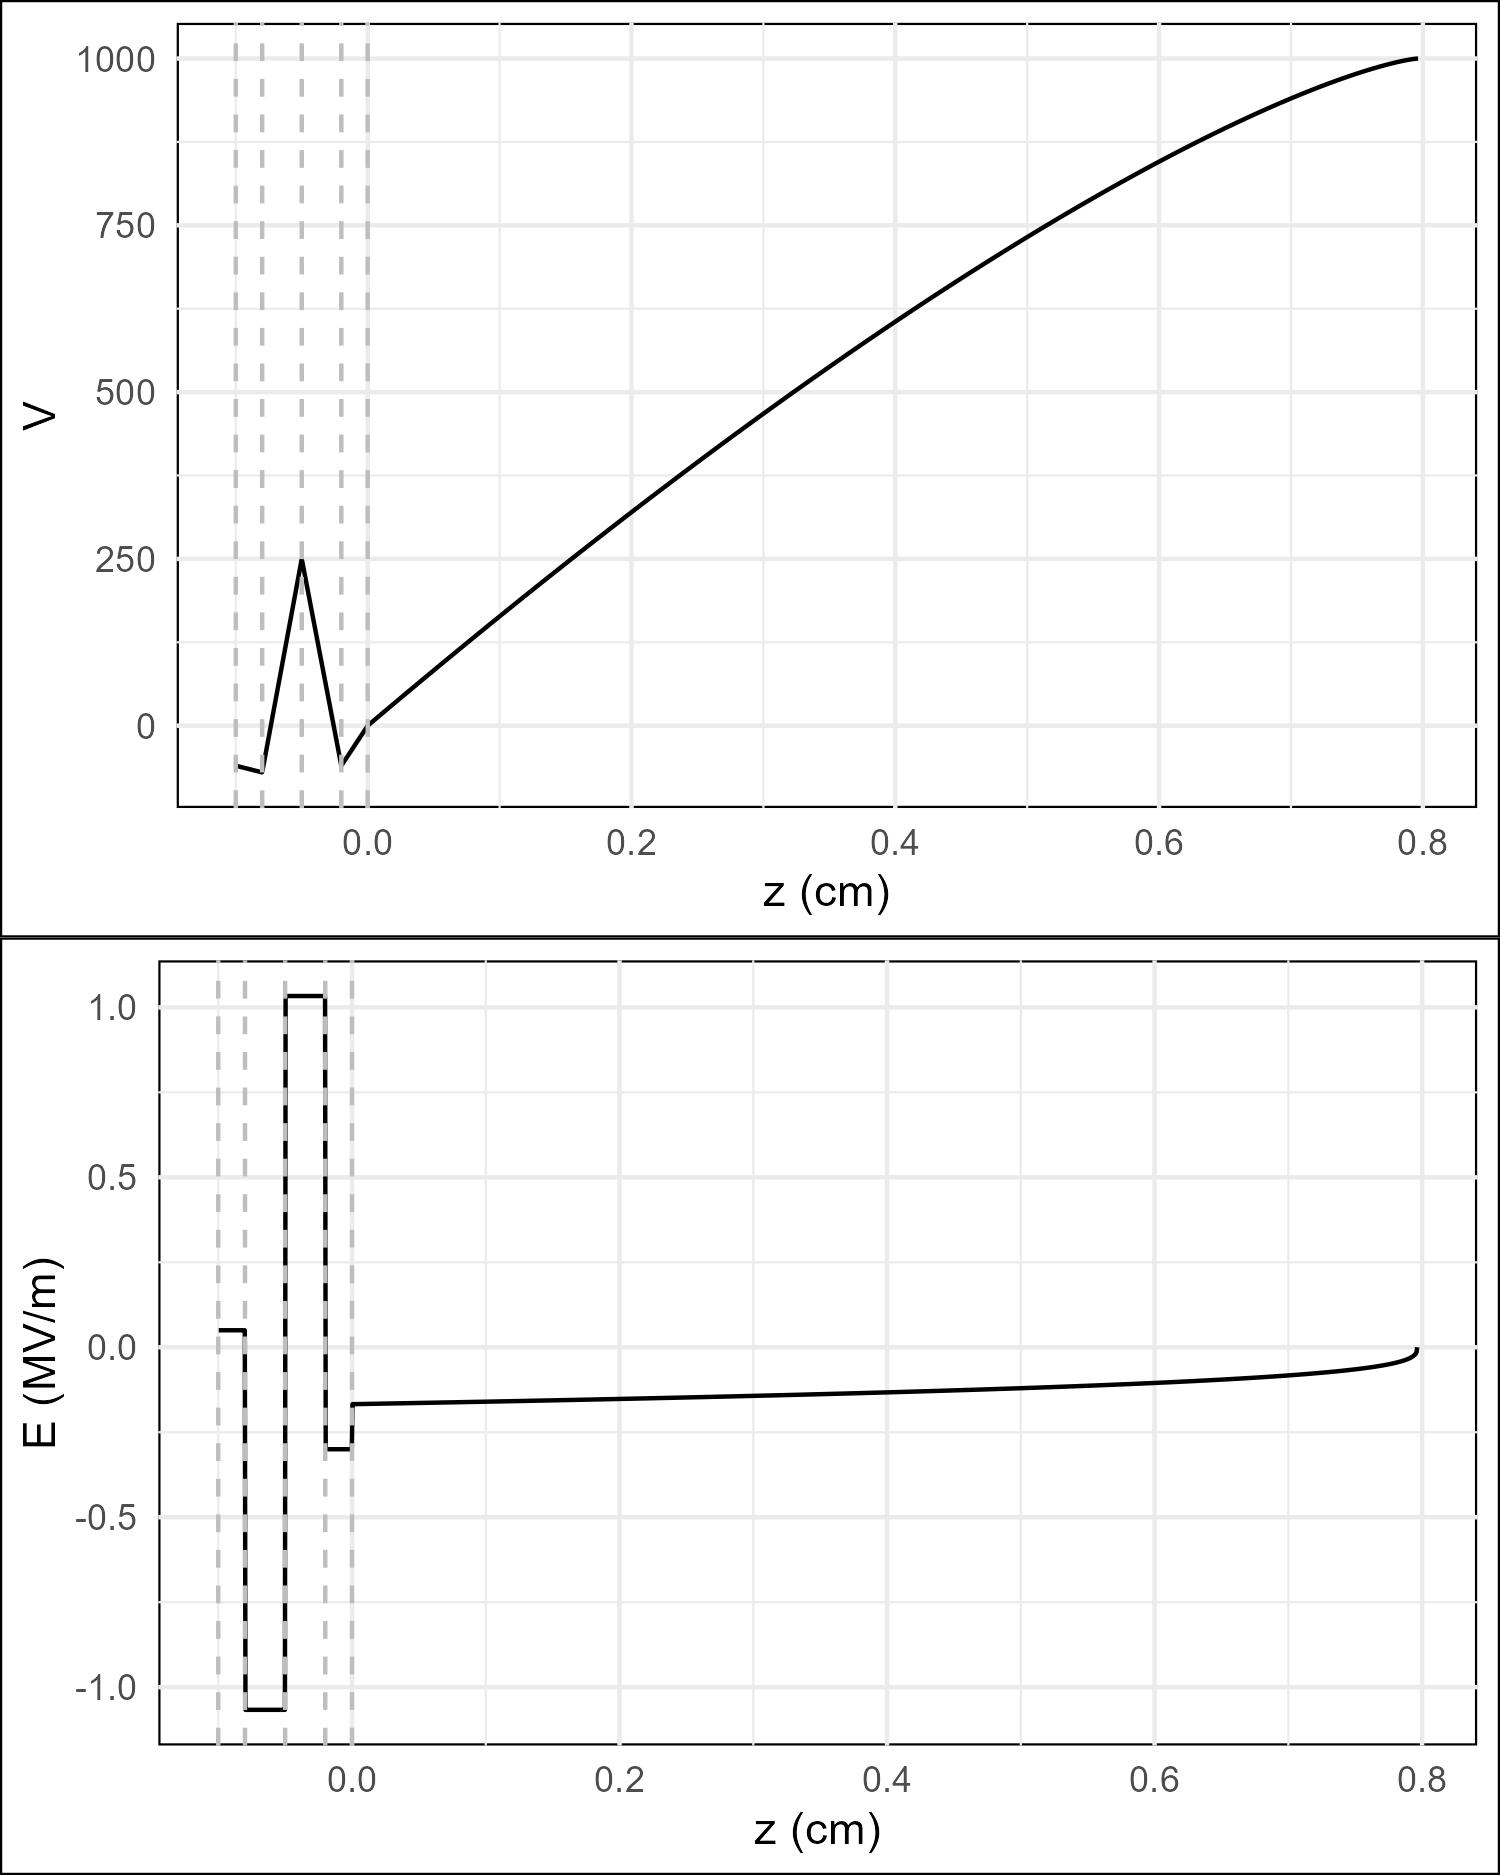
\includegraphics[width=0.45\textwidth]{Figures/VEz2DC1kVStack2332.jpeg}
\caption{Space potential across a plasma sheath and RFEA grid stack (top) and corresponding electric field (bottom) for DC plasma sheath with a voltage across the sheath of 1000~V. The edge of the plasma sheath and plasma is at $z=0.8$~cm. The RFEA is located at $z\le0$; with the plasma facing grid (G$_0$) at $z=0$. The location of the RFEA grids and collector are indicated by vertical dashed lines.}
\label{fig:DCpotentialField}
\end{figure}



The space potential and electric field for the AC sheath are calculated using the capacitive sheath solution of reference~\cite{Lieberman1988}. The sheath edge of the capacitive radio-frequency discharge changes through the cycle, from collapsing when the voltage across the sheath drops to its minimum to full expansion when the voltage is maximum. The size of the sheath is given by, 
\begin{eqnarray}
s(\phi) &=& s_0 ( 1 - \cos(\phi) + \frac{H}{8} \{ \frac32 \sin(\phi)  + \frac{11}{18} \sin(3 \phi) \nonumber \\ 
        & & - 3 \phi \cos(\phi)  - \frac13 \phi \cos(3 \phi)  \} )
\end{eqnarray}
With $\phi = \omega t$ ($\omega = 2 \pi f$) and $f$ the radio-frequency. The value of $s(t)$ is limited to $\phi$ in the range from 0 ($t=0$) to $\pi$ ($t=T/2$; where $T=1/f$ is the radio-frequency cycle period). The size of the sheath at $t=0$ is zero and its maximum size at $s(t=T/2) = s_m$. The $s(t)$ function can be evaluated at any time value via the following 
\begin{eqnarray}
s(t)    &=& \text{abs}(s(\omega \tau(t))) \\
\tau(t) &=& \text{remainder}\left(\frac{t}{T}+\frac12\right) - \frac{T}{2} 
\end{eqnarray}
The parameter $s_0$ is given by 
\begin{equation}
s_0 = \frac{J}{e n_s \omega}
\end{equation}
$J$ is the total current through the plasma discharge (mainly displacement current in the sheaths and conduction current in the plasma bulk). The current can be calculated from the plasma density at the sheath edge ($n_s$) and the maximum voltage across the sheath ($V_0$)
\begin{equation}
J = \frac25 \omega \sqrt{\frac65} \sqrt{e n_s \epsilon_0 (\sqrt{576+125 V_0}-24)}
\end{equation}
The $H$ parameter is given by
\begin{equation}
H = \frac1{\pi} \frac{s_0^2}{\lambda_D^2}
\end{equation}

The electric field in the z-direction is given by 
\begin{equation}
E_{AC}(z,t) = \frac{J}{\epsilon_0 \omega} \left \{ \cos(\omega t) - \cos(\phi(s_m - z)) \right \} 
\end{equation}
If $s(t)<s_m-z$, otherwise the electric field is zero. Note that the function $\phi(s)$ is the inverse of the sheath size $s(\phi)$, that it does not have an analytical solution, and that it is numerically solved in the computer code. 

Finally, the space potential for the capacitive radio-frequency sheath is given by the integral
\begin{equation}
V_{AC}(z,t) = \int_{0}^{z} E_{AC}(z\prime, t) dz\prime
\end{equation}
With $z$ in the range from $z=0$ to $z=s_m$. The field is numerically integrated.  




\subsection{\label{IonTrajectory}Ion trajectory integration}

\subsection{\label{IonCollision}Collisions of ions with background gas}

